\documentclass[aps,prd,twocolumn,nofootinbib,superscriptaddress,10pt]{revtex4-2}

\usepackage{amsmath,amssymb,bm}
\usepackage{graphicx}
\usepackage{booktabs}
\usepackage[colorlinks=true,linkcolor=blue,citecolor=blue,urlcolor=blue]{hyperref}

\newcommand{\ii}{\mathrm{i}}
\newcommand{\dd}{\mathrm{d}}
\newcommand{\calO}{\mathcal{O}}
\newcommand{\rp}{r_+}
\newcommand{\rmn}{r_-}
\newcommand{\OmH}{\Omega_H}
\newcommand{\Bin}{B^{\rm inc}}
\newcommand{\Bref}{B^{\rm ref}}
\newcommand{\Aref}{A_{\rm ref}^{(1)}}
\newcommand{\AH}{A_H^{(1)}}
\newcommand{\W}{\mathcal{W}}

\begin{document}

\title{Nonlinear scalar scattering on Kerr from an endpoint spectral Green-function method}

\author{KerrScattering Project}
\affiliation{Manuscript draft generated from the KerrScattering repository}

\date{\today}

\begin{abstract}
We formulate and compute the leading weakly nonlinear scattering response of a
self-interacting complex scalar field on Kerr.  The calculation is the rotating
black-hole continuation of a Schwarzschild nonlinear Green-function spectral
method.  The scalar Teukolsky equation is solved in the compact coordinate
$z=\rp/r$, with infinity and the future horizon retained as collocation
endpoints.  After peeling the known phases, the degenerate endpoint rows of the
radial equation provide regular first-order boundary conditions.  The linear
horizon-normalized in mode is matched to down/up solutions at an intermediate
radius to obtain $\Bin$ and $\Bref$.  Against 37 scalar
GeneralizedSasakiNakamura.jl benchmark cases, the worst invariant amplitude
error is $1.485\times10^{-8}$ and the worst flux residual is
$3.714\times10^{-9}$.  For a cubic interaction
$\Box\Phi+\epsilon|\Phi|^2\Phi=0$, the Kerr factor
$\Sigma=r^2+a^2\cos^2\theta$ generates a projected radial source
$(r^2C^{(0)}_{\ell'\ell m}+a^2C^{(2)}_{\ell'\ell m})|R_{\ell m}|^2R_{\ell m}$.
We compute the first-order Green-function amplitudes for self and target
channels, including a representative $\ell'=2,\ldots,6$ channel scan for
$(a,\ell,m,M\omega)=(0.5,2,2,0.30)$.  For the self channel, converting the
unit-horizon response to fixed incident normalization gives
$T^{(1)}+R^{(1)}\simeq0$, the Kerr analogue of the nonlinear balance law in
the Schwarzschild problem.  Off-diagonal target channels are nonzero at the
field-amplitude level but enter energy flux only at quadratic order in the
nonlinear correction.
\end{abstract}

\maketitle

\section{Introduction}

Scattering by black holes provides observables complementary to quasinormal
mode spectra.  In linear theory, scalar, electromagnetic, and gravitational
waves on Schwarzschild and Kerr backgrounds exhibit barrier penetration,
greybody factors, superradiance, and resonance structures which are well
understood through partial waves and related complex-angular-momentum
methods~\cite{Taylor,Futterman,Teukolsky1973,StarobinskyChurilov,PressTeukolsky,GlampedakisAndersson,Dolan2008}.
These quantities are also relevant for recent frequency-domain descriptions of
black-hole ringdowns in terms of greybody factors rather than only sums of
quasinormal modes~\cite{Oshita2022,Rosato2024}.

The nonlinear scattering problem is less developed.  The Schwarzschild
calculation used as the template for the present work considers a weak
self-interaction and computes the first nonlinear correction by feeding the
linear in solution into a Green-function source.  Its central structure is
simple: solve the homogeneous scattering problem accurately, project the
nonlinear source onto partial waves, impose no incoming nonlinear radiation,
and read off the first-order correction to the horizon and infinity fluxes.

Here we carry this strategy to the scalar Teukolsky equation on Kerr, keeping
the same computational philosophy as the Schwarzschild spectral code.  The new
features are genuinely Kerr-specific.  First, the angular basis is spheroidal,
not spherical.  Second, the radial equation contains the horizon frequency
$p=\omega-m\OmH$, so the linear flux law allows superradiant reflection.
Third, the nonlinear source is not merely a spherical Gaunt coefficient times a
radial power: multiplying the equation by
$\Sigma=r^2+a^2\cos^2\theta$ produces two angular projectors and couples the
source mode $(\ell,m)$ to target channels $\ell'$ of the same $m$.

The paper follows the structure of the Schwarzschild nonlinear Green-function
template.  Section~\ref{sec:setup} defines the nonlinear Kerr scalar
scattering problem.  Section~\ref{sec:methods} describes the endpoint spectral
method and the nonlinear Green-function amplitudes.  Section~\ref{sec:results}
reports the linear validation, superradiant frequency sweep, nonlinear
self-channel balance, and the first target-channel matrix result.

\section{Nonlinear scattering problem on Kerr}
\label{sec:setup}

\subsection{Scalar Teukolsky equation}

In Boyer--Lindquist coordinates,
\begin{align}
\Sigma &= r^2+a^2\cos^2\theta,\\
\Delta &= r^2-2Mr+a^2=(r-\rp)(r-\rmn),\\
\rp &= M+\sqrt{M^2-a^2},\qquad
\rmn = M-\sqrt{M^2-a^2},
\end{align}
and
\begin{equation}
\OmH=\frac{a}{\rp^2+a^2}.
\end{equation}
We use the Kerr tortoise coordinate
\begin{equation}
\frac{\dd r_*}{\dd r}=\frac{r^2+a^2}{\Delta}.
\end{equation}
The additive constant in $r_*$ fixes only an overall scattering phase.

For the scalar mode
\begin{equation}
\Phi_{\ell m\omega}^{(0)}
 =
R_{\ell m\omega}(r)S_{\ell m}(\theta;a\omega)
e^{\ii m\phi-\ii\omega t},
\end{equation}
the angular equation is
\begin{align}
0={}&
\frac{1}{\sin\theta}\frac{\dd}{\dd\theta}
\left(\sin\theta\frac{\dd S_{\ell m}}{\dd\theta}\right)
\notag\\
&+
\left[
a^2\omega^2\cos^2\theta
-\frac{m^2}{\sin^2\theta}
+A_{\ell m}
\right]S_{\ell m},
\end{align}
with unit normalization on the sphere.  The radial equation is
\begin{equation}
\frac{\dd}{\dd r}
\left(\Delta\frac{\dd R_{\ell m\omega}}{\dd r}\right)
+
\left(\frac{K^2}{\Delta}-\lambda_{\ell m\omega}\right)
R_{\ell m\omega}=0,
\label{eq:radial}
\end{equation}
where
\begin{equation}
K=(r^2+a^2)\omega-am,\qquad
\lambda_{\ell m\omega}=A_{\ell m}+a^2\omega^2-2am\omega .
\end{equation}
For $a\omega=0$, $S_{\ell m}$ reduces to the spherical harmonic and
$\lambda=\ell(\ell+1)$.

\subsection{Linear boundary conditions and fluxes}

The horizon-normalized in solution is defined by
\begin{equation}
R_{\ell m\omega}^{\rm in}\sim e^{-\ii p r_*},
\qquad p=\omega-m\OmH,\qquad r\rightarrow \rp ,
\end{equation}
and at infinity by
\begin{equation}
R_{\ell m\omega}^{\rm in}\sim
\Bin_{\ell m\omega}\frac{e^{-\ii\omega r_*}}{r}
+
\Bref_{\ell m\omega}\frac{e^{+\ii\omega r_*}}{r}.
\label{eq:linearbc}
\end{equation}
With this convention the incident amplitude is $\Bin$, the reflected amplitude
is $\Bref$, and the horizon transmission amplitude is unity.  The invariant
linear reflection and transmission factors for a unit incident wave are
\begin{equation}
R^{(0)}=\left|\frac{\Bref}{\Bin}\right|^2,
\qquad
T^{(0)}=\frac{p(\rp^2+a^2)}{\omega|\Bin|^2},
\label{eq:linearRT}
\end{equation}
so that
\begin{equation}
T^{(0)}+R^{(0)}=1.
\end{equation}
When $p<0$, $T^{(0)}<0$ and the reflected flux exceeds the incident flux:
this is scalar superradiance.

\subsection{Weak cubic source}

We take the self-interacting scalar equation to be
\begin{equation}
\Box\Phi+\epsilon|\Phi|^2\Phi=0,\qquad |\epsilon|\ll1,
\end{equation}
and expand
\begin{equation}
\Phi=\Phi^{(0)}+\epsilon\Phi^{(1)}+\calO(\epsilon^2).
\end{equation}
For a monochromatic source mode $(\ell,m,\omega)$, the cubic term has the same
time and azimuthal dependence.  We therefore write
\begin{equation}
\Phi^{(1)}
=
e^{\ii m\phi-\ii\omega t}
\sum_{\ell'\ge |m|}
R_{\ell'|\ell m\omega}^{(1)}(r)S_{\ell'm}(\theta;a\omega).
\end{equation}
Multiplying the scalar wave equation by $\Sigma$ and projecting onto the target
spheroidal harmonic gives
\begin{equation}
\mathcal{L}_{\ell'}R_{\ell'|\ell m\omega}^{(1)}
=-Q_{\ell'\ell m}(r),
\label{eq:sourceeq}
\end{equation}
where $\mathcal{L}_{\ell'}$ denotes the radial operator in
Eq.~\eqref{eq:radial} with $\lambda_{\ell'm\omega}$, and
\begin{equation}
Q_{\ell'\ell m}(r)=
\left[
r^2 C^{(0)}_{\ell'\ell m}
+a^2 C^{(2)}_{\ell'\ell m}
\right]
|R_{\ell m\omega}^{\rm in}|^2R_{\ell m\omega}^{\rm in}.
\label{eq:Q}
\end{equation}
The two angular projectors are
\begin{equation}
C^{(s)}_{\ell'\ell m}
=
\int \dd\Omega\,
\cos^s\theta\,
S^*_{\ell'm}|S_{\ell m}|^2S_{\ell m},
\qquad s=0,2 .
\label{eq:C}
\end{equation}
This is the first structural difference from the Schwarzschild calculation:
even a single incident spheroidal mode sources a target-channel matrix.

\section{Methods}
\label{sec:methods}

\subsection{Endpoint pseudo-spectral homogeneous solutions}

We solve Eq.~\eqref{eq:radial} on two Chebyshev subdomains in
\begin{equation}
z=\frac{\rp}{r},\qquad z=0\leftrightarrow r=\infty,\qquad
z=1\leftrightarrow r=\rp .
\end{equation}
The known phases are peeled off before discretization,
\begin{align}
R_{\rm in}&=e^{-\ii p r_*}u_{\rm in}(z),\\
R_{\rm down}&=\frac{e^{-\ii\omega r_*}}{r}u_{\rm down}(z),\\
R_{\rm up}&=\frac{e^{+\ii\omega r_*}}{r}u_{\rm up}(z).
\end{align}
The transformed equation has the schematic form
\begin{equation}
B_2(z)u''(z)+B_1(z)u'(z)+B_0(z)u(z)=0.
\end{equation}
At $z=0$ for down/up modes and at $z=1$ for the in mode, $B_2$ vanishes.
Thus the endpoint row is a first-order regularity condition rather than an
externally imposed truncation.  The normalizations are
\begin{equation}
u_{\rm down}(0)=1,\qquad u_{\rm up}(0)=1,\qquad u_{\rm in}(1)=1.
\end{equation}
For low frequencies we use an analytic sinh mapping to cluster points toward
the far-field endpoint, following the same motivation as the Schwarzschild
Gevrey-regularity discussion in the base calculation.

At an intermediate point $z_m=\rp/r_m$, the horizon solution is matched to
down/up solutions:
\begin{equation}
R_{\rm in}=
\Bin R_{\rm down}+\Bref R_{\rm up}.
\label{eq:match}
\end{equation}
Matching both $R$ and $\dd R/\dd r$ gives the linear amplitudes.

\subsection{Green-function nonlinear amplitudes}

Let $R_{\ell'm\omega}^{\rm in}$ and $R_{\ell'm\omega}^{\rm up}$ denote the
target-channel in and up solutions.  The radial Wronskian
\begin{equation}
\W_{\ell'}=
\Delta
\left(
R_{\ell'}^{\rm in}\frac{\dd R_{\ell'}^{\rm up}}{\dd r}
-
R_{\ell'}^{\rm up}\frac{\dd R_{\ell'}^{\rm in}}{\dd r}
\right)
\label{eq:W}
\end{equation}
is independent of $r$.  The first-order solution is required to contain no
incoming nonlinear radiation from infinity and no outgoing nonlinear radiation
from the past horizon.  The two Green-function amplitudes are therefore
\begin{align}
A_{{\rm ref},\ell'|\ell m}^{(1)}
&=
-\frac{1}{\W_{\ell'}}
\int_{\rp}^{\infty}
R_{\ell'}^{\rm in}(r) Q_{\ell'\ell m}(r)\,\dd r,
\label{eq:Aref}\\
A_{H,\ell'|\ell m}^{(1)}
&=
-\frac{1}{\W_{\ell'}}
\int_{\rp}^{\infty}
R_{\ell'}^{\rm up}(r) Q_{\ell'\ell m}(r)\,\dd r.
\label{eq:AH}
\end{align}
These are the quantities directly computed by the code in unit-horizon
normalization.

The outer part of the integrals is highly oscillatory.  On the outer domain,
$R_{\rm in}$ is a sum of down and up phases, while $R_{\rm up}$ is outgoing.
The products in Eqs.~\eqref{eq:Aref} and~\eqref{eq:AH} decompose into
phase channels $\exp(\ii n\omega r_*)$ with $n=-4,-2,0,2,4$.  We integrate
the exterior tail in $r_*$ with Fourier-weighted quadrature, while the inner
finite interval is integrated by Gauss-Legendre quadrature in $z$.

\subsection{Fixed incident normalization and nonlinear balance}

The amplitudes in Eqs.~\eqref{eq:Aref} and~\eqref{eq:AH} correspond to a
linear solution with unit horizon transmission.  To compare with the
Schwarzschild nonlinear scattering coefficients, we fix the incident amplitude
to unity.  The rescaled field is
\begin{equation}
R_{\rm phys}^{(0)}=\alpha R_{\rm in},\qquad \alpha=\frac{1}{\Bin}.
\end{equation}
Since the source is cubic, the first-order field scales as
$|\alpha|^2\alpha$.  For the self channel $\ell'=\ell$, the physical reflected
and horizon amplitudes are
\begin{align}
\mathcal{R}_{\rm phys}
&=
\frac{\Bref}{\Bin}
+
\epsilon\,\frac{\Aref}{|\Bin|^2\Bin},
\\
\mathcal{H}_{\rm phys}
&=
\frac{1}{\Bin}
+
\epsilon\,\frac{\AH}{|\Bin|^2\Bin}.
\end{align}
The first nonlinear corrections to the flux coefficients are
\begin{align}
R^{(1)}
&=
\frac{2\,\mathrm{Re}\left[\left(\Bref\right)^*\Aref\right]}
{|\Bin|^4},
\label{eq:R1}\\
T^{(1)}
&=
\frac{2p(\rp^2+a^2)}{\omega|\Bin|^4}
\mathrm{Re}\,\AH .
\label{eq:T1}
\end{align}
For a self-channel source, conservation implies
\begin{equation}
T^{(1)}+R^{(1)}=0,
\label{eq:nonlinearbalance}
\end{equation}
up to numerical error.  Off-diagonal target channels are orthogonal to the
linear outgoing channel in the angular integral.  They are first-order field
amplitudes, but their direct energy-flux contribution starts at
$\calO(\epsilon^2)$.

\section{Results}
\label{sec:results}

\subsection{Linear validation and superradiance}

The linear solver was validated against GeneralizedSasakiNakamura.jl in the
unit-Teukolsky-transmission convention~\cite{GSN}.  Complex phases were not
used as pass/fail quantities because a shift of the Kerr tortoise coordinate
changes them.  The benchmark gates were imposed on $|\Bin|$, $|\Bref|$, and
the flux balance.

\begin{table}[b]
\caption{Linear scalar validation summary.  The benchmark grid contains
Schwarzschild, moderate-spin, high-spin, superradiant, and non-superradiant
cases.}
\begin{ruledtabular}
\begin{tabular}{l c}
quantity & value\\
\hline
usable GSN benchmark cases & 37\\
frequency-sweep points & 51\\
worst amplitude-magnitude error & $1.485\times10^{-8}$\\
worst flux residual & $3.714\times10^{-9}$\\
largest sampled superradiant gain & $4.970\times10^{-4}$\\
\end{tabular}
\end{ruledtabular}
\label{tab:linear}
\end{table}

\begin{figure*}[t]
\centering
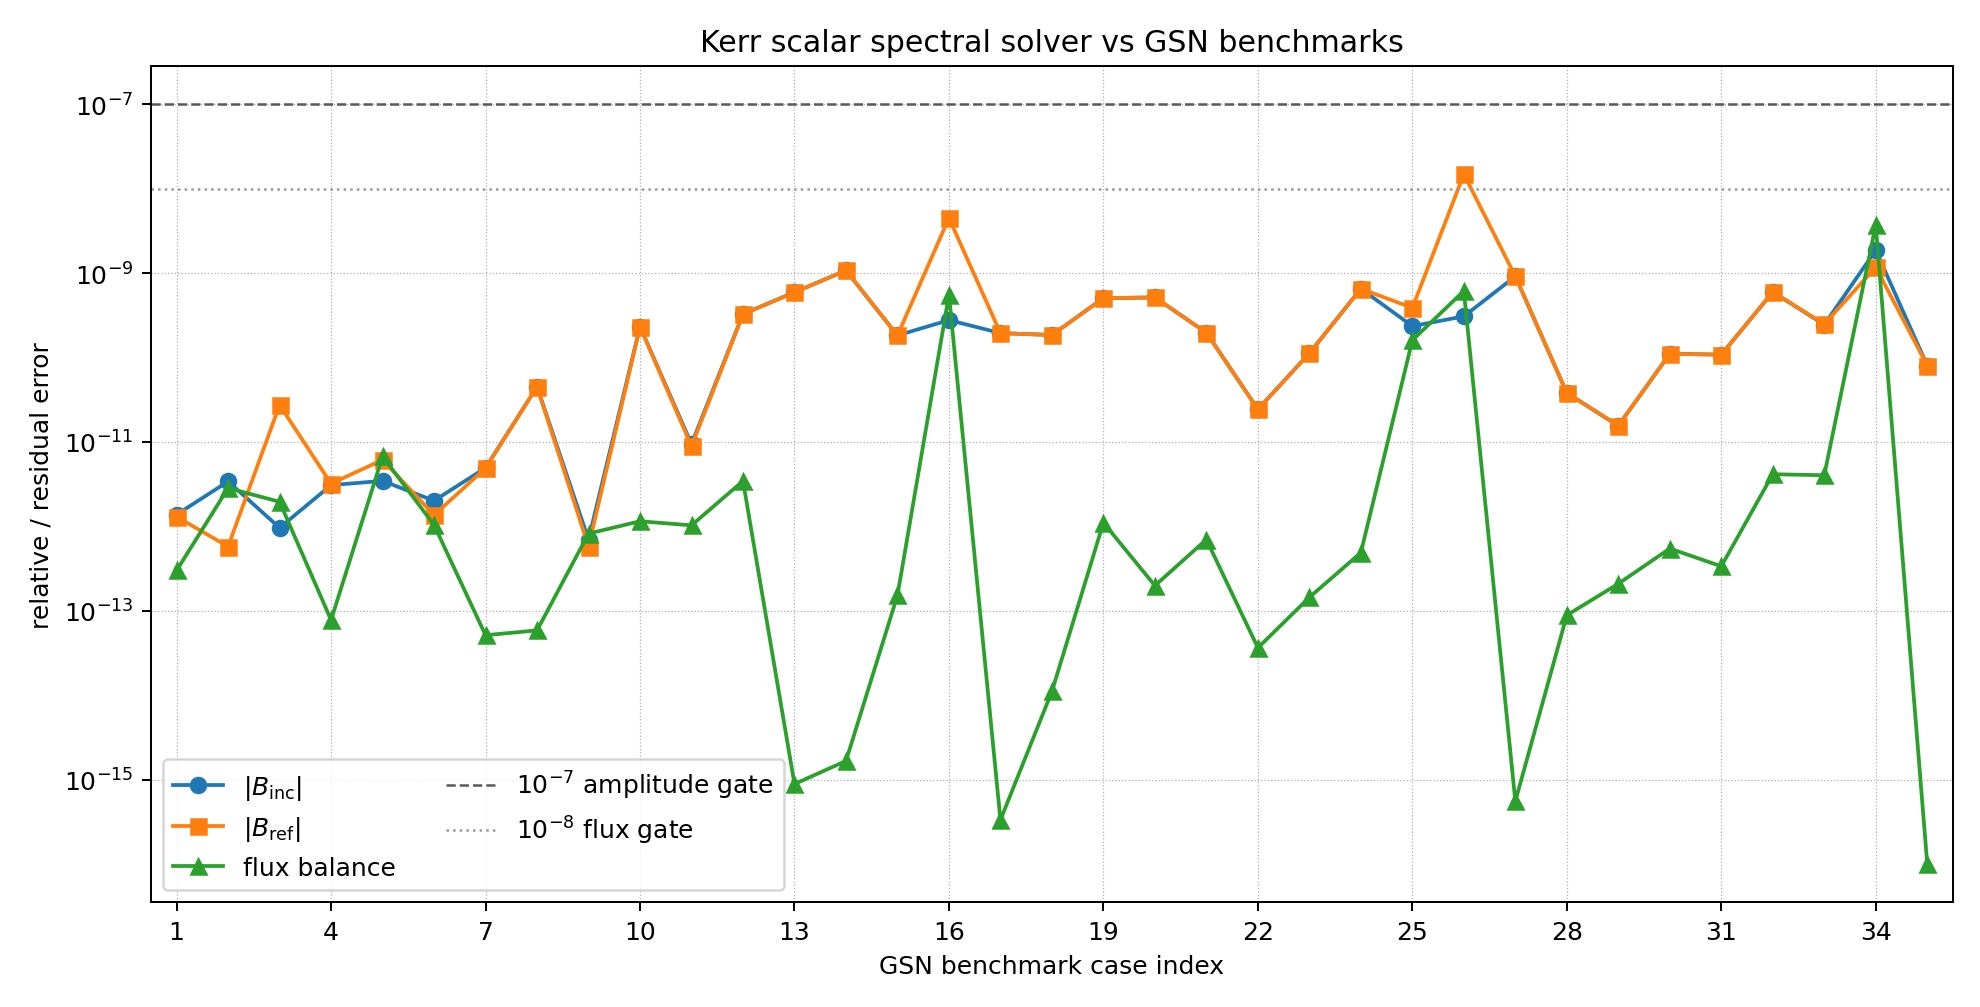
\includegraphics[width=0.47\textwidth]{../../figures/kerr_scalar_adaptive_errors.png}
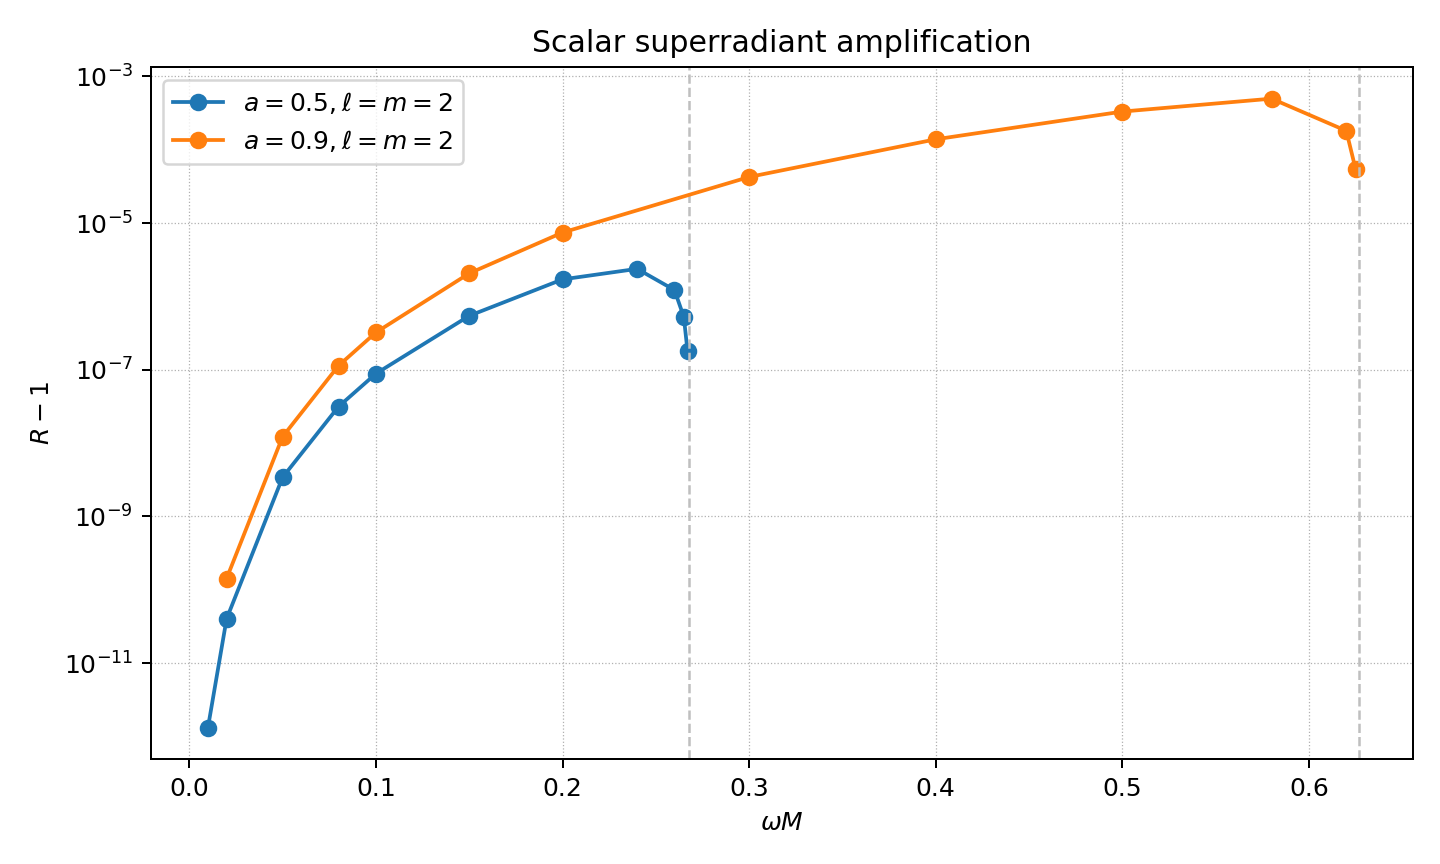
\includegraphics[width=0.47\textwidth]{../../figures/kerr_scalar_superradiance_amplification.png}
\caption{Linear validation.  Left: invariant benchmark errors against
GeneralizedSasakiNakamura.jl.  Right: frequency sweep showing scalar Kerr
superradiant amplification only for $\omega<m\OmH$.}
\label{fig:linear}
\end{figure*}

\subsection{Self-channel nonlinear flux coefficients}

Table~\ref{tab:flux} gives the fixed-incident self-channel coefficients of
Eqs.~\eqref{eq:R1} and~\eqref{eq:T1}.  The Schwarzschild row is included as a
limit check against the base problem.  For ordinary absorption
($p>0$), a positive cubic coupling in the present sign convention increases
the transmitted flux and decreases the reflected flux.  In the superradiant
regime ($p<0$), $T^{(0)}<0$ and the signs reverse in the same flux-balance
sense.

\begin{table*}[t]
\caption{Self-channel nonlinear flux coefficients in fixed incident
normalization.  The source model is Eq.~\eqref{eq:Q}; computations use
$N=288$, $q=224$, and Fourier-tail tolerance $10^{-11}$.}
\begin{ruledtabular}
\begin{tabular}{l c c c c c}
case & $M\omega$ & $T^{(0)}$ & $R^{(0)}$ & $T^{(1)}$ & $R^{(1)}$\\
\hline
Schwarzschild $\ell=0$ & $0.10$ & $3.245\times10^{-1}$ & $6.755\times10^{-1}$
& $8.726\times10^{-2}$ & $-8.726\times10^{-2}$\\
Kerr $a=0.5,\ell=m=2$ superradiant & $0.24$ & $-2.373\times10^{-6}$
& $1.000002373$ & $-2.153\times10^{-7}$ & $2.039\times10^{-7}$\\
Kerr $a=0.5,\ell=m=2$ absorbing & $0.30$ & $1.595\times10^{-5}$
& $9.999840\times10^{-1}$ & $1.582\times10^{-6}$ & $-1.582\times10^{-6}$\\
Kerr $a=0.9,\ell=m=2$ superradiant & $0.58$ & $-4.970\times10^{-4}$
& $1.000497031$ & $-7.819\times10^{-5}$ & $7.819\times10^{-5}$\\
\end{tabular}
\end{ruledtabular}
\label{tab:flux}
\end{table*}

The nonlinear balance residual $T^{(1)}+R^{(1)}$ is
$3.3\times10^{-12}$ for the Schwarzschild row,
$-5.6\times10^{-13}$ for the absorbing Kerr $a=0.5$ row, and
$-2.7\times10^{-13}$ for the high-spin superradiant row.  The
$a=0.5$, $M\omega=0.24$ row is closer to the superradiant threshold and shows
a larger absolute residual, $-1.1\times10^{-8}$, because the two nonlinear
flux terms are obtained from large nearly cancelling Green-function
amplitudes.

\subsection{Target-channel matrix}

For the representative absorbing Kerr mode
$(a,\ell,m,M\omega)=(0.5,2,2,0.30)$, the cubic source was projected onto
target channels $\ell'=2,\ldots,6$.  Odd target channels vanish by angular
parity in this case.  The production computation used $N=288$, $q=224$, and
Fourier-tail tolerance $10^{-11}$.

\begin{table}[b]
\caption{Unit-horizon first-order Green-function amplitudes for the first Kerr
target-channel scan.}
\begin{ruledtabular}
\begin{tabular}{c c c c}
$\ell'$ & $|C^{(0)}_{\ell'\ell m}|$ &
$|A_{{\rm ref},\ell'|\ell m}^{(1)}|$ & $|A_{H,\ell'|\ell m}^{(1)}|$\\
\hline
2 & $1.136\times10^{-1}$ & $1.137\times10^{6}$ & $3.804\times10^{3}$\\
3 & $0$ & $0$ & $0$\\
4 & $3.578\times10^{-2}$ & $1.362\times10^{4}$ & $1.319$\\
5 & $0$ & $0$ & $0$\\
6 & $5.341\times10^{-3}$ & $2.265\times10^{3}$ & $5.383\times10^{-7}$\\
\end{tabular}
\end{ruledtabular}
\label{tab:channels}
\end{table}

\begin{figure*}[t]
\centering
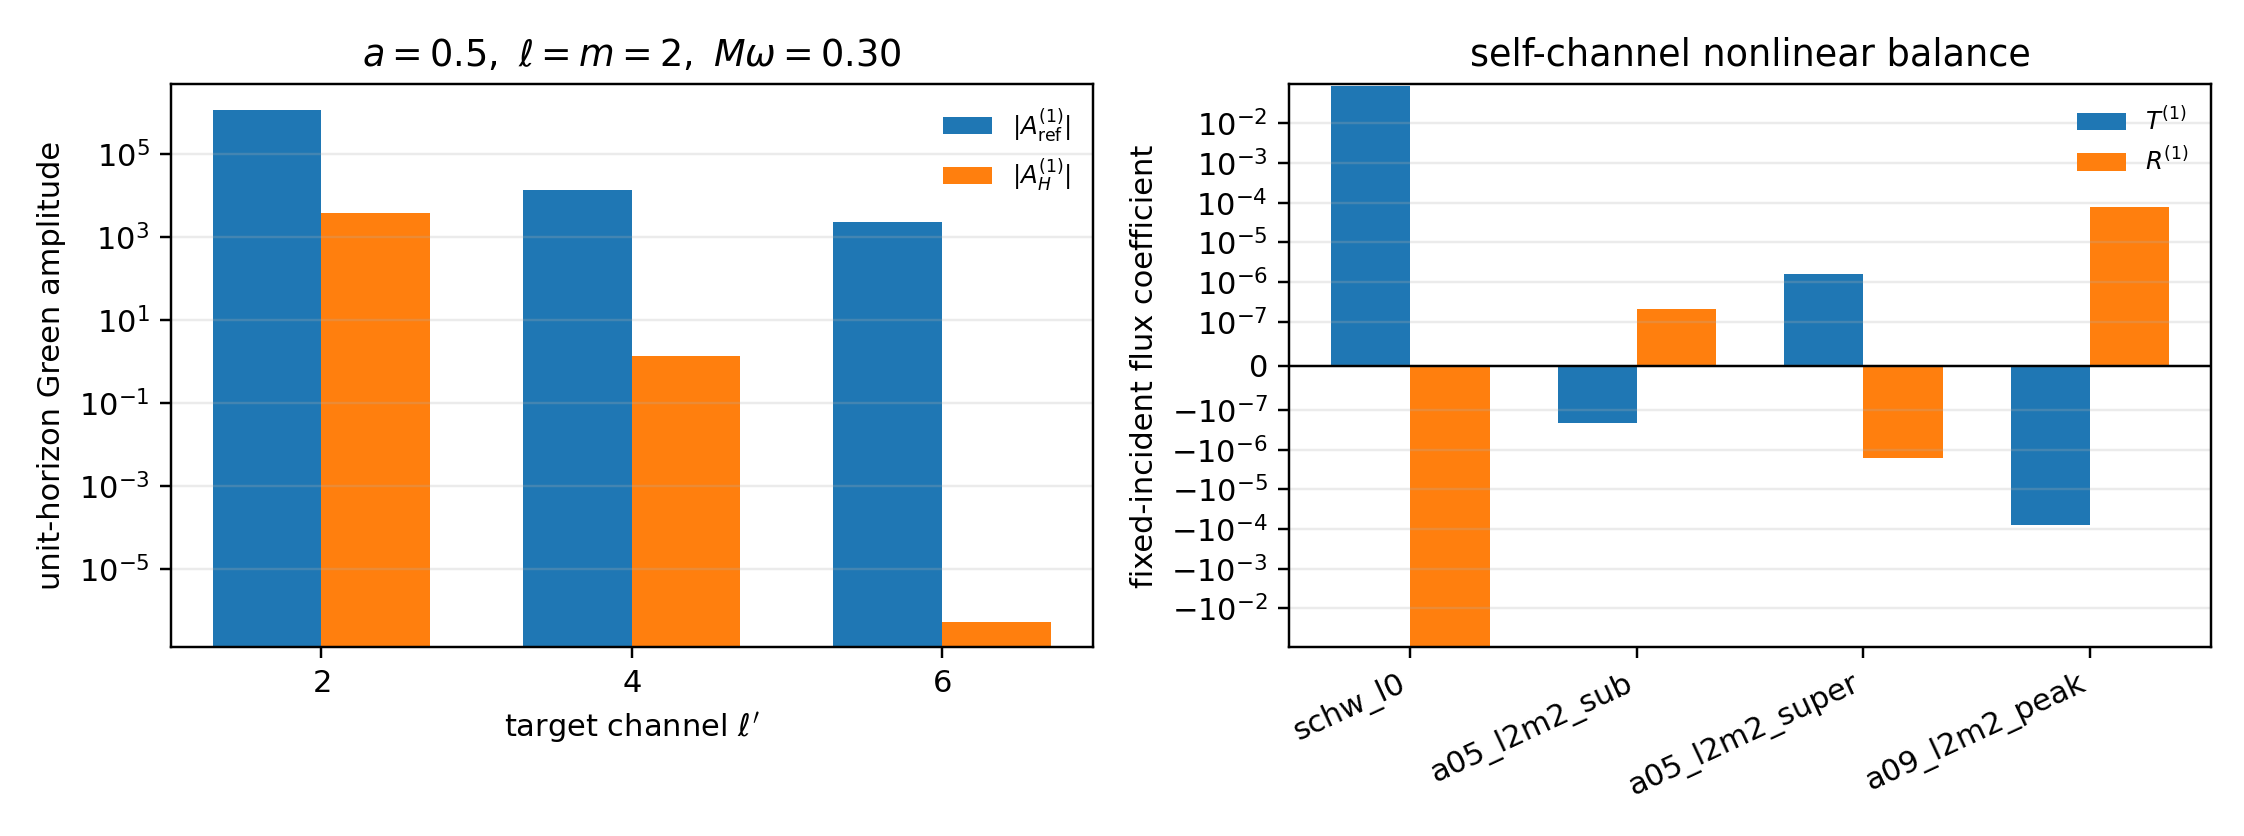
\includegraphics[width=0.95\textwidth]{../../figures/kerr_scalar_nonlinear_results.png}
\caption{Nonlinear Kerr scalar results.  Left: unit-horizon Green-function
amplitudes in the first active target-channel scan.  Right: fixed-incident
self-channel nonlinear flux coefficients.  A symmetric logarithmic scale is
used in the right panel to show both superradiant and absorbing cases.}
\label{fig:nonlinear}
\end{figure*}

A fixed-$q=224$ convergence scan over $N=224,256,288$ gives a largest
reflected-amplitude change of $1.14\times10^{-4}$ relative to the $N=288$
reference row, while the change from $N=256$ to $N=288$ is at most
$6.27\times10^{-7}$ over the active reflected channels.  The off-diagonal
horizon amplitudes are more cancellation limited.  The $\ell'=4$ horizon
amplitude is stable at roughly the percent level between $N=256$ and $N=288$,
whereas $\ell'=6$ is a near-zero $10^{-7}$ quantity and should be interpreted
only as an order-of-magnitude diagnostic at current double precision.

\section{Discussion and next steps}

The central conclusion is that the Schwarzschild nonlinear Green-function
workflow extends cleanly to Kerr scalar scattering once the spheroidal angular
projection and the Kerr flux normalization are handled explicitly.  The linear
piece is already benchmarked to the level required for a production solver.
The nonlinear self-channel reproduces the expected first-order flux balance
after converting from unit-horizon to fixed incident normalization.  The Kerr
geometry also exposes a new object absent from the simple Schwarzschild
self-channel calculation: the target-channel amplitude matrix
$A_{{\rm ref},\ell'|\ell m}^{(1)}$ and $A_{H,\ell'|\ell m}^{(1)}$.

The present results should be read with two normalization caveats.  First, the
tabulated Green amplitudes are not by themselves physical nonlinear
corrections; the physical field correction is $\epsilon A^{(1)}$, and fixed
incident normalization introduces the cubic scaling in
Eqs.~\eqref{eq:R1}--\eqref{eq:T1}.  Second, off-diagonal first-order fields do
not interfere with the linear outgoing field in the angular flux, so their
energy contribution starts at $\calO(\epsilon^2)$.

The immediate numerical extensions are therefore clear: broaden the
target-channel scan over $(a,\ell,m,\omega)$, set acceptance gates for the
off-diagonal horizon amplitudes, and replace or cross-check the QUADPACK
Fourier-tail integral with a dedicated Levin or Filon oscillatory integrator.

\appendix

\section{Schwarzschild limit}

For $a=0$, $\rp=2M$, $\OmH=0$, $S_{\ell m}$ reduces to $Y_{\ell m}$, and
Eq.~\eqref{eq:radial} is equivalent to the Regge--Wheeler scalar equation for
the master variable $\psi=rR$:
\begin{equation}
\begin{aligned}
\left[
\frac{\dd^2}{\dd r_*^2}
+\omega^2
-f\left(\frac{\ell(\ell+1)}{r^2}+\frac{2M}{r^3}\right)
\right]\psi&=0,\\
f&=1-\frac{2M}{r}.
\end{aligned}
\end{equation}
The source Eq.~\eqref{eq:Q} becomes
$r^2C^{(0)}_{\ell'\ell m}|R|^2R$.  In the master variable this is the familiar
$r^{-2}$ cubic radial weight of the Schwarzschild nonlinear Green-function
problem.  Thus the Kerr implementation reduces to the base method when
$a=0$, while retaining the endpoint-collocation boundary treatment.

\begin{thebibliography}{99}

\bibitem{Taylor}
J. R. Taylor,
\textit{Scattering Theory: The Quantum Theory of Nonrelativistic Collisions}
(John Wiley and Sons, New York, 1972).

\bibitem{Futterman}
J. A. H. Futterman, F. A. Handler, and R. A. Matzner,
\textit{Scattering from Black Holes}
(Cambridge University Press, Cambridge, 2012).

\bibitem{Teukolsky1973}
S. A. Teukolsky,
Perturbations of a rotating black hole. I. Fundamental equations for
gravitational, electromagnetic, and neutrino-field perturbations,
Astrophys. J. \textbf{185}, 635 (1973).

\bibitem{StarobinskyChurilov}
A. A. Starobinsky and S. M. Churilov,
Amplification of electromagnetic and gravitational waves scattered by a
rotating black hole,
Sov. Phys. JETP \textbf{38}, 1 (1974).

\bibitem{PressTeukolsky}
W. H. Press and S. A. Teukolsky,
Floating orbits, superradiant scattering and the black-hole bomb,
Nature \textbf{238}, 211 (1972).

\bibitem{GlampedakisAndersson}
K. Glampedakis and N. Andersson,
Scattering of scalar waves by rotating black holes,
Class. Quant. Grav. \textbf{18}, 1939 (2001).

\bibitem{Dolan2008}
S. R. Dolan,
Scattering and absorption of gravitational plane waves by rotating black holes,
Class. Quant. Grav. \textbf{25}, 235002 (2008).

\bibitem{Oshita2022}
N. Oshita,
Thermal ringdown of a Kerr black hole: overtone excitation, Fermi-Dirac
statistics and greybody factor,
JCAP \textbf{04}, 013 (2023).

\bibitem{Rosato2024}
R. F. Rosato, K. Destounis, and P. Pani,
Ringdown stability: Graybody factors as stable gravitational-wave observables,
Phys. Rev. D \textbf{110}, L121501 (2024).

\bibitem{GSN}
R. K. L. Lo,
GeneralizedSasakiNakamura.jl,
\url{https://github.com/ricokaloklo/GeneralizedSasakiNakamura.jl}.

\end{thebibliography}

\end{document}
